\chapter{Le Projet}

\section{Règles du jeu}
Le jeu est composé d'un plateau formé grâce à 4 quarts de plateau à 2 faces ce qui permet d'obtenir 96 configurations différentes. Le plateau est un quadrillage de 16 par 16 cases dont certaines sont des cases objectif. 

À chaque tour, le ou les joueur(s) reçoivent l'objectif à atteindre. Le but est alors d'amener le robot de la couleur correspondante sur la case objectif dont le symbole est identique à celui de l'objectif. Si l'objectif est multicolore, il faut alors amener n'importe quel robot sur la case multicolore du plateau.

Les joueurs jouent simultanément, chacun réfléchissant sur le moyen d'amener le robot en utilisant les règles de déplacement. Lorsque l'un d'entre eux pense avoir trouvé une solution, il annonce en combien de mouvements il compte atteindre l'objectif puis il active le compte à rebours de 120 secondes. Les autres joueurs ont jusqu'à la fin du compte à rebours pour proposer de meilleures solutions, utilisant moins de mouvements.
Après l'écoulement du temps, le joueur qui a la solution comptant le moins de mouvement montre sa solution et remporte la tuile. S'il échoue dans sa démonstration, le joueur qui proposait le nombre de mouvements immédiatement supérieur montre sa solution, etc. jusqu'à ce qu'une solution soit valide.

\section{Analyse de l'existant}
Le projet consistant à implémenter un jeu de société, nous avons commencé par en étudier les règles. Nous avons donc étudié le jeu original Rasende Roboter. Nous avons ensuite recherché s'il existait une version libre d'un projet similaire au notre. Nous avons fini par trouver plusieurs implémentations différentes (tant par le langage choisi que par la modification des règles originales).
Nous avons notamment trouvé le code développé par une équipe de l'INSA de Rouen qui nous a permis de nous faire une idée générale de ce que nous avions à coder.

\section{Manuel de l'application}
\begin{figure}[!h]
	\centering
   	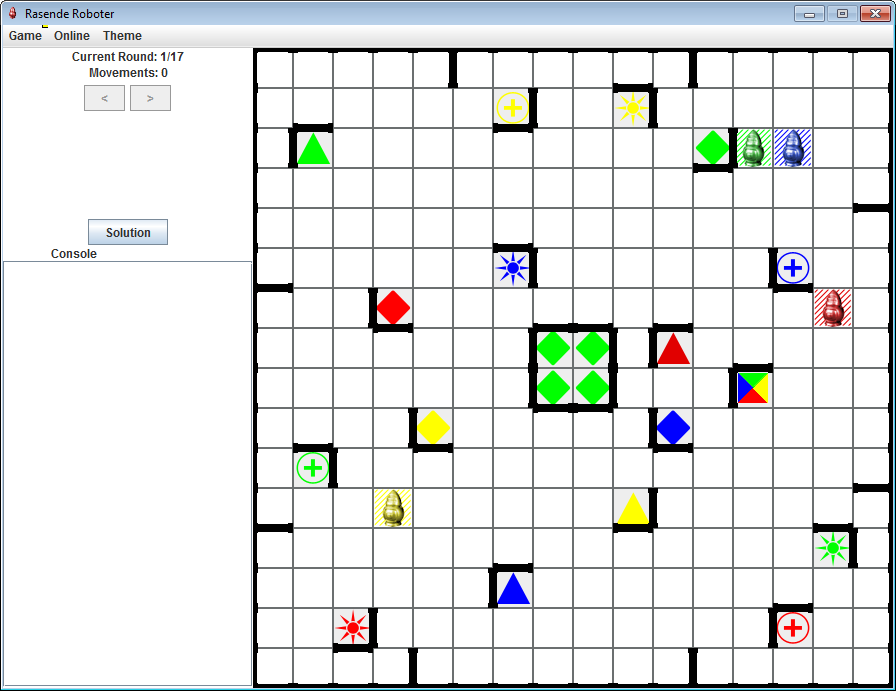
\includegraphics[scale=0.5]{img/interfacegraphique.png}
	\caption{Interface graphique de notre Rasende Roboter}
\end{figure}
Le jeu possède trois composantes importantes : la barre de menu, le panneau de contrôle et le plateau de jeu.

\subsection{Barre de menu}
Le menu "Game" permet de lancer une nouvelle partie en cliquant sur "New Game". Un nouveau plateau de jeu est alors généré avec un nouvel objectif et le compteur de tour est réinitialisé.
En cliquant sur "Help", les règles et le fonctionnement du jeu vous seront rappelés.
Cliquer sur "License" affichera les crédits du jeu, c'est-à-dire les développeurs du jeu, ainsi que la licence utilisée pour le créer.
Pour quitter le jeu il faut cliquer sur le bouton "Quit".
 
Le menu "Online" permet de se mesurer à d'autres joueurs en rejoignant un serveur déjà créé, ou en en créant un soi-même.
Pour rejoindre un serveur, cliquez sur "Join server". Il vous sera alors demandé un nom d'utilisateur ainsi que l'IP du serveur à rejoindre.
 
Pour créer son propre serveur et pouvoir accueillir d'autres joueurs dans votre partie, cliquez sur "Start Server". Seul un nom d'utilisateur vous sera demandé.

Le menu "Theme" vous permettra de choisir entre deux thèmes graphiques : le thème par défaut et le thème Pokemon. D'autres thèmes peuvent facilement être rajoutés si besoin.

\subsection{Panneau de contrôle}
Le panneau de contrôle permet de suivre la progression du jeu et d'effectuer des actions.
\subsubsection{En partie locale}
"Current Round" indique le tour qui est joué.
"Movements" indique le nombre de déplacements qui ont été fait avec les robots pendant le tour actuel.
Le chevron "\textless" permet d'annuler le dernier mouvement effectué et le chevron "\textgreater" permet de rétablir un mouvement qui a été annulé.
Le bouton "Solution" lance un solveur qui calcule le chemin le plus rapide pour arriver sur l'objectif et affiche les déplacements nécessaires dans la console. Il est ensuite affiché dans la console.
\subsubsection{En partie en ligne}
Si la partie en cours est en ligne, les informations disponibles dans le panneau de contrôle ne sont pas exactement les mêmes.
Pour commencer, afin d'éviter la triche, le bouton de solution disparait de la colonne. En revanche, la liste des joueurs connectés et le nombre de point apparaît. Il est aussi possible de proposer son estimation du nombre de coups que l'on prévoit de faire. Le premier joueur qui valide son estimation lance un compteur pendant lequel tout le monde peut proposer son estimation. Une fois que le compteur se termine, les joueurs sont classés selon leur estimation et celui qui a la plus petite prend la main pour montrer le chemin qu'il a trouvé. S'il n'y arrive pas il peut abandonner le tour en cliquant sur "Forfeit" et laisse alors la main au joueur suivant et ainsi de suite ...

\subsection{Le plateau de jeu et déplacement des robots}
\begin{figure}[!h]
   	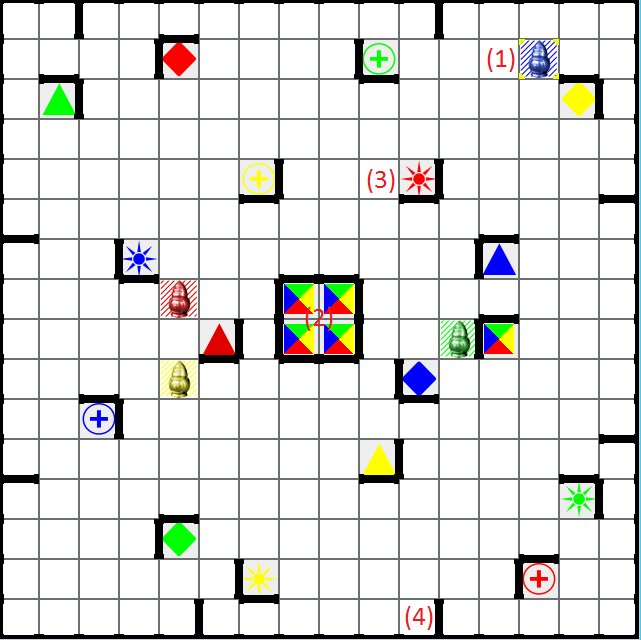
\includegraphics[scale=0.5]{img/plateaudejeu.png}
   	\centering
	\caption{Capture du plateau de jeu pendant un partie}
	Le plateau est un quadrillage contenant les 4 pions, l'objectif, les cases cibles avec leurs murs.
	\begin{enumerate}
		\item Un des quatre pions du jeu. Les cases de départ des pions sont marquées par des rayures de la couleur du robot. Le robot sélectionné est encadré en jaune.
		\item L'objectif à atteindre par les robots.
		\item Une case cible.
		\item Les murs sont représentés par des traits noirs épais.
	\end{enumerate}
\end{figure}

Les robots se déplacent de manière rectiligne jusqu'à rencontrer un obstacle (mur ou autre robot). En partie locale, on peut bouger les robots quand on veut, en revanche en partie en ligne on peut bouger les robots seulement si on a la main.
Il faut d'abord sélectionner un robot. Soit en cliquant dessus soit en utilisant le clavier avec les touches :
\begin{itemize}
	\item R ou 1 pour le robot rouge
	\item V ou 2 pour le robot vert
	\item B ou 3 pour le robot bleu
	\item Y ou 4 pour le robot jaune
\end{itemize}
Ensuite utilisé les flèches directionnelles ou la souris pour déplacer le robot sélectionné dans l'une des quatre directions possibles.



\subsection{Conseils}
En premier lieu, vous apprendrez clairement beaucoup plus de choses en jouant plutôt qu'en lisant cette rubrique qui sera forcément très courte. 
N'oubliez pas que vous pouvez utiliser tous les robots. 
Vérifiez rapidement s'il n'existe pas un chemin direct entre le robot et son objectif (une solution en 6 ou 7 coups). 
Si ce n'est pas le cas, regardez quelles sont les possibilités pour arriver sur la bonne case et quels robots vous pouvez placer en obstacle pour y arriver.
Vous vous êtes trompés en déplaçant un robot ? Utilisez les boutons "<" et ">" pour revenir en arrière ou inversement.
Lors d'une partie en ligne, n'oubliez pas que vous pouvez faire des annonces supérieures à celles déjà faites, le joueur a pu se tromper.
Les solutions en plus de 15 coups sont rares, mais ça arrive. Ce sont évidemment des solutions qui demandent une grande concentration pour être trouvée. Si personne ne trouve de solution (chaque problème à une solution), n'hésitez pas à passer le tour. 
Évitez d'enchaîner les parties, c'est un jeu qui fatigue vite.
